\documentclass{article}

\usepackage{color}
\usepackage{xcolor}
\usepackage{alltt}
\usepackage{tikz}
\usepackage{bm}

\usepackage[breakable]{tcolorbox} % for text box
\usepackage{graphicx} % for minipage
\usepackage[margin=2cm]{geometry} % margins
\usetikzlibrary{bayesnet}

\begin{document}
\begin{tcolorbox}[breakable, width=\textwidth, colback=gray!10, boxrule=0pt,
  title=simpleYule.lphy, fonttitle=\bfseries]

\begin{minipage}[t]{0.50\textwidth}
\section*{Code}

\small
\begin{alltt}
model \{
  \textcolor{green}{\(\lambda\)} ~ \textcolor{blue}{LogNormal}(\textcolor{gray}{meanlog=}\textcolor{magenta}{3.0}, \textcolor{gray}{sdlog=}\textcolor{magenta}{1.0});
  \textcolor{green}{\(\psi\)} ~ \textcolor{blue}{Yule}(\textcolor{gray}{lambda=}\textcolor{green}{\(\lambda\)}, \textcolor{gray}{n=}\textcolor{magenta}{16});
  \textcolor{green}{D} ~ \textcolor{blue}{PhyloCTMC}(\textcolor{gray}{L=}\textcolor{magenta}{200}, \textcolor{gray}{Q=}\textcolor{magenta!80!black}{jukesCantor}(), \textcolor{gray}{tree=}\textcolor{green}{\(\psi\)});
\}
\end{alltt}
\section*{Model}

The alignment, {\it D} is assumed to have evolved under a phylogenetic continuous time Markov process \cite{Felsenstein1981Evolutionary} on  phylogenetic time tree, $\psi$, with an instantaneous rate matrix and a length of 200.
The instantaneous rate matrix is the Jukes-Cantor model \cite{Jukes1969Evolution}.
The phylogenetic time tree, $\psi$ is assumed to come from a Yule \cite{Yule1925II.} with  lambda, $\lambda$ and an n of 16.
The lambda, $\lambda$ has a log-normal prior with a mean in log space of 3.0 and a standard deviation in log space of 1.0.

\section*{Posterior}

The posterior distribution is:

$$P(\psi, \lambda | \textrm{D}) \propto P(\textrm{D} | \psi) P(\psi | \lambda) P(\lambda) $$
\end{minipage}
\begin{minipage}[t]{0.50\textwidth}
\section*{Graphical Model}

\begin{center}
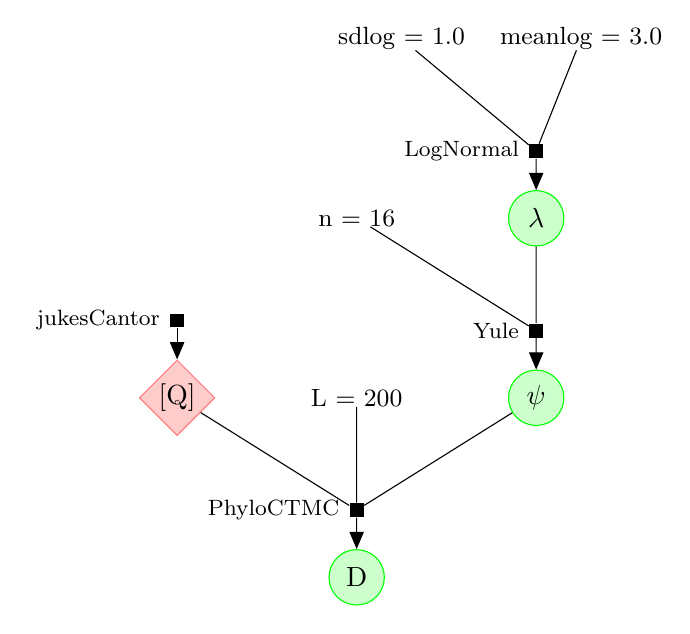
\begin{tikzpicture}[scale=0.95,
dstyle/.style={draw=blue!50,fill=blue!20},
vstyle/.style={draw=green,fill=green!20},
cstyle/.style={font=\small},
detstyle/.style={draw=red!50,fill=red!20}
]
\node[const, cstyle] at (3.0, -0.0) (2110299480) {sdlog = 1.0};
\node[const, cstyle] at (5.3999999999999995, -0.0) (1306292113) {meanlog = 3.0};
\node[const, cstyle] at (2.4, -2.4) (676470331) {n = 16};
\node[latent, vstyle] at (4.8, -2.4) (lambda) {$\lambda$};
\node[det, detstyle] at (0.0, -4.8) (1075680047) {[Q]};
\node[const, cstyle] at (2.4, -4.8) (1135326386) {L = 200};
\node[latent, vstyle] at (4.8, -4.8) (psi) {$\psi$};
\node[latent, vstyle] at (2.4, -7.199999999999999) (D) {D};
\factor[above=of lambda] {LogNormallambda} {left:LogNormal} {} {} ; %
\factoredge {1306292113, 2110299480} {LogNormallambda} {lambda}; %
\factor[above=of 1075680047] {jukesCantor1075680047} {left:jukesCantor} {} {} ; %
\factoredge {} {jukesCantor1075680047} {1075680047}; %
\factor[above=of psi] {Yulepsi} {left:Yule} {} {} ; %
\factoredge {lambda, 676470331} {Yulepsi} {psi}; %
\factor[above=of D] {PhyloCTMCD} {left:PhyloCTMC} {} {} ; %
\factoredge {1135326386, 1075680047, psi} {PhyloCTMCD} {D}; %
\end{tikzpicture}
\end{center}
\begin{thebibliography}{9}

\bibitem{Felsenstein1981Evolutionary}
Felsenstein, J. (1981). Evolutionary trees from DNA sequences: a maximum likelihood approach. Journal of molecular evolution, 17(6), 368-376.

\bibitem{Jukes1969Evolution}
Jukes, T. H., \& Cantor, C. R. (1969). Evolution of protein molecules. Mammalian protein metabolism, 3, 21-132.

\bibitem{Yule1925II.}
Yule, G. U. (1925). II.� A mathematical theory of evolution, based on the conclusions of Dr. JC Willis, FRS. Philosophical transactions of the Royal Society of London. Series B, containing papers of a biological character, 213(402-410), 21-87.

\end{thebibliography}
\end{minipage}
\end{tcolorbox}

\end{document}
